%\documentclass[onecolumn]{IEEEtranTIE}
\documentclass[journal]{IEEEtranTIE}

\usepackage{graphicx}
\usepackage{cite}
\usepackage{picinpar}
\usepackage{amsmath}
\usepackage{url}
\usepackage{flushend}
\usepackage[latin1]{inputenc}
\usepackage{colortbl}
\usepackage{soul}
\usepackage{multirow}
\usepackage{pifont}
\usepackage{color}
\usepackage{alltt}
\usepackage[hidelinks]{hyperref}
\usepackage{enumerate}
\usepackage{siunitx}
\usepackage{breakurl}
\usepackage{epstopdf}
\usepackage{pbox}

\usepackage{booktabs}
\usepackage{amsmath}
\usepackage{amssymb}
\usepackage{amsthm}
\usepackage{bm}
\usepackage{todonotes}
\usepackage{tikz}
\usepackage{pgfplots}
\usepackage[section]{algorithm}
\usepackage{algorithmicx}
\usepackage{algpseudocode}
\renewcommand{\algorithmicrequire}{\textbf{Input:}}
\renewcommand{\algorithmicensure}{\textbf{Output:}}
\algnewcommand\Offline{\item[\textbf{Offline:}]}

\newtheorem{thm}{Theorem}[section]
\newtheorem{theorem}[thm]{Theorem}
\newtheorem{lemma}[thm]{Lemma}
\newtheorem{proposition}[thm]{Proposition}
\theoremstyle{definition}
\newtheorem{definition}[thm]{Definition}
\newtheorem{example}[thm]{Example}

\newcommand{\R}{{\mathbb R}}
\newcommand{\mnmz}{\operatorname*{minimize}}
\newcommand{\mxmz}{\operatorname*{maximize}}
\newcommand{\argmin}{\operatorname{argmin}}
\newcommand{\argmax}{\operatorname{argmax}}
\newcommand{\stt}{\operatorname{subject\ to}}
\newcommand{\nrm}[1]{|#1|}
\newcommand{\norm}[1]{\|#1\|}
\newcommand{\rank}{\operatorname{rank}}


\begin{document}
\title{	Preparation of Papers for IEEE Trans on Industrial Electronics \\ (Nov. 2020)}

\author{
	\vskip 1em
	
	First A. Author1, \emph{Student Membership},
	Second B. Author2, \emph{Membership},
	\\ and Third C. Author3, \emph{Membership}

	\thanks{
	
		Manuscript received Month xx, 2xxx; revised Month xx, xxxx; accepted Month x, xxxx.
		This work was supported in part by the xxx Department of xxx under Grant  (sponsor and financial support acknowledgment goes here).
		
		(Authors' names and affiliation) First A. Author1 and Second B. Author2 are with the xxx Department, University of xxx, City, Zip code, Country, on leave from the National Institute for xxx, City, Zip code, Country (e-mail: author@domain.com). 
		
		Third C. Author3 is with the National Institute of xxx, City, Zip code, Country (corresponding author to provide phone: xxx-xxx-xxxx; fax: xxx-xxx-xxxx; e-mail: author@ domain.gov).
	}
}

\maketitle
	
\begin{abstract}
Paper titles should be written in uppercase and lowercase letters, not all uppercase. Avoid writing long formulas with subscripts in the title; short formulas that identify the elements are fine (e.g., ``Nd-Fe-B''). Do not write ``(Invited)'' in the title. Write full names of authors in the author field. Define all symbols used in the abstract. Do not cite references in the abstract. Do not delete the blank line immediately above the abstract; it sets the footnote at the bottom of this column.
\end{abstract}

\begin{IEEEkeywords}
??? Enter key words or phrases in alphabetical order, separated by commas.
\end{IEEEkeywords}

\markboth{IEEE TRANSACTIONS ON INDUSTRIAL ELECTRONICS}%
{}

\definecolor{limegreen}{rgb}{0.2, 0.8, 0.2}
\definecolor{forestgreen}{rgb}{0.13, 0.55, 0.13}
\definecolor{greenhtml}{rgb}{0.0, 0.5, 0.0}

\section{Important information}

\IEEEPARstart{T}{his} ???

Regular Papers and Special Section papers - Four to eight pages, including authors' bios and photos.

\begin{enumerate}[1)]
	\item New manuscripts cannot exceed \textbf{8 pages} (3 for letters). Only a very limited overlength (1/2 page at most) is tolerated. Note that usually in the review process the reviewers tend to ask for more explanations, also note that the maximum allowed length is 8 pages on initial/first submission, including authors' bios and photos.
	\item In order to follow the \textbf{single-blind} review process, we ask that all the authors be identifiable within the manuscript (DO include authors' names, their biographies, affiliation, etc.). Each published article was reviewed by a minimum of two independent reviewers using a single-blind peer review process.
	\item The only file which has to be submitted (uploaded) is the \textbf{manuscript in PDF format}.
	\item IEEE T IE is an application oriented engineering journal. It is therefore expected that all submissions will \textbf{contain experimental verification} of the novel theoretical concepts, given in the paper. Papers not containing experimental results should therefore not be submitted since they will be subject to an ``Immediate reject'' decision. An experimental rig, which must be used by the authors for verification, must contain hardware components other than a PC/laptop.	
\end{enumerate}

Figures that are composed of only black lines and shapes. These figures should have no shades or half-tones of gray. Only black and white.

The final printed size of author photographs is exactly
1 inch wide by 1.25 inches tall (25.4 millimeters x 31.75 millimeters / 6 picas x 7.5 picas).

When referencing your figures and tables within your paper, use the abbreviation ``Fig.'' even at the beginning of a sentence. Do not abbreviate ``Table.'' Tables should be numbered with Roman Numerals.

The IEEE Graphics Checker Tool enables authors to pre-screen their graphics for compliance with IEEE Transactions and Journals standards before submission. The online tool, located at \url{http://graphicsqc.ieee.org/}, allows authors to upload their graphics in order to check that ... 

A conclusion section is not required. Although a conclusion may review the main points of the paper, do not replicate the abstract as the conclusion. A conclusion might elaborate on the importance of the work or suggest applications and extensions.

Reference numbers are set flush left and form a column of their own, hanging out beyond the body of the reference. The reference numbers are on the line, enclosed in square brackets. In all references, the given name of the author or editor is abbreviated to the initial only and precedes the last name. Use them all; use et al. exceptionally if more than 6 author names were listed. Use commas around Jr., Sr., and III in names. 

Other than books \cite{inbook1, book1, book2, book3}, capitalize only the first word in a paper title, except for proper nouns and element symbols. 

Because replication is required for scientific progress, papers submitted for publication must provide sufficient information to allow readers to perform similar experiments or calculations and use the reported results. Although not everything need be disclosed, a paper must contain new, useable, and fully described information.

\newpage





\section{Introduction}

Pokus

Text of the introduction.
\begin{itemize}
\item minimum effort control - minimizing the control effort, where the
effort is defined as maximum amplitude of the control \cite{neustadt1962minimum,porter1966note,Tomlin1975}
\item minimum effort control in robotics (kinematically redundant manipulators)
\cite{ajoudani2013human,lee2001structured,Shim1998,Lee&Ha2001}, 
\item traditional control methods of power converters, carrier-based PWM
techniques (sinusoidal, TIPWM) and space vector-based techniques (SVPWM).
\end{itemize}

\section{Motivation and principles}

\subsection{Redundant Voltage Source Network }

The problem of redundant voltage source network, degrees of freedom.
Analogy to voltage source converters. Clarke's transform, A matrix,
vector x as a vector of final voltages with minimum amplitudes.

\begin{equation}
\begin{aligned}x=\left[\cdots\right]{}^{T},\\
A=\left[\cdots\right],
\end{aligned}
\label{eq:eq2-1}
\end{equation}
Motivation -> minimize voltage needed.

\subsection{Optimization problem definition}

Linear system, minimum infinity norm, solution vector x. Primal problem
definition...

\begin{equation}
\min_{\mathbf{Ax}=\mathbf{y}}||\mathbf{x}||_{\text{\ensuremath{\infty}}},\label{eq:1}
\end{equation}


\subsection{Solution using linear programming???}

Note sure if this is to include in the paper......Solution using linear
programming - linprog() in Matlab environment, suitable for mathematical
modeling and rapid method development for any type of converter. Not
effective for real-time application...

\section{Proposed Solution}

\subsection{Solution way for $m\times(m + 1)$ matrices}


If matrix $A$ is of size $m\times(m+1)$ and if its rank is $m$ (its rows are independent), then we have
$$
  \{x\mid Ax=y\} = \{x^0 + sa\mid s\in\R\},
$$
where $x^0$ is an arbitrary point which satisfies $Ax^0=y$ and $a$ is a nonzero element of kernel of A (it satisfies $Aa=0$). Then \eqref{eq:primal} is equivalent to
$$
  \aligned
  \mnmz_{x,s}\ &\norm{x}_\infty \\
  \stt\ &x = x^0 + sa,
  \endaligned
$$ 
which amounts solving an optimization problem in one dimension
\begin{equation}\label{eq:problem}
  \aligned
  \mnmz_{s}\ &\norm{x^0+sa}_\infty.
  \endaligned
\end{equation}

For the the optimal solution of \eqref{eq:problem}, there will be some indices $i\neq j$ such that the components satisfy
$$
  (x^0+sa)_i = \pm(x^0+sa)_j.
$$
This have two solutions (if properly defined)
$$
  \aligned
  s^1 &= \frac{-x^0_i+x_j^0}{a_i-a_j}, \\
  s^2 &= \frac{-x^0_i-x_j^0}{a_i+a_j}.
  \endaligned
$$
Then among all these $s$, we select the one with minimal $\norm{x^0+sa}_\infty$. We summarize the procedure in Algorithm \ref{alg1}.

\begin{algorithm}
  \caption{For solving \eqref{eq:primal} with one degree of freedom}
  \label{alg1}
  \begin{algorithmic}[1]
    \State Find some nonzero $\bm a$ such that $A\bm a=0$
    \State Find some $\bm x^0$ such that $A\bm x^0=\bm y$
    \State $f_{\rm min} \gets \infty$
    \For {$i$ in $1:m+1$}
    \For {$j$ in $i+1:m+1$}
    \If {$a_i\neq a_j$}
    \State $s \gets \frac{-x^0_i+x_j^0}{a_i-a_j}$
    \If {$\norm{\bm x^0 + s\bm a}_\infty \le f_{\rm min}$}
    \State $f_{\rm min} \gets \norm{\bm x^0 + s\bm a}_\infty$
    \State $s_{\rm opt} \gets s$
    \EndIf
    \EndIf
    \If {$a_i\neq -a_j$}
    \State $s \gets \frac{-x^0_i-x_j^0}{a_i+a_j}$
    \If {$\norm{\bm x^0 + s\bm a}_\infty \le f_{\rm min}$}
    \State $f_{\rm min} \gets \norm{\bm x^0 + s\bm a}_\infty$
    \State $s_{\rm opt} \gets s$
    \EndIf
    \EndIf
    \EndFor
    \EndFor
  \end{algorithmic}
\end{algorithm}


\todo[inline]{What is the complexity of the algorithm?}

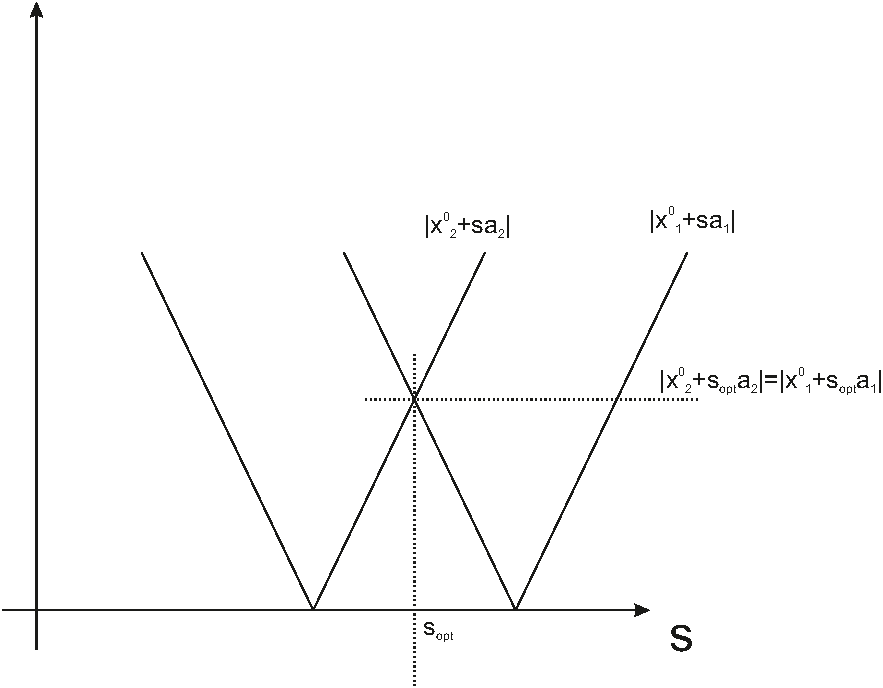
\includegraphics[width=0.9\columnwidth]{Figures/ilust_obr_x0+sa}



\subsection{Solution way for a general matrix $A$}

... Duality of $\ell_{1}$ and $\ell_{\infty}$ norm (D. G. Luenberger)
\cite{Luenberger1997optimization}. Dual problem defined by Cadzow:

The Cadzow algorithm \cite{Cadzow1973,Cadzow1974efficient} is based
on a solution search of the associated dual problem 
\begin{equation}
\max_{\left\Vert \mathbf{A}^{T}\mathbf{u}\right\Vert _{1}\leqq1}\mathbf{y}^{T}\mathbf{u}=\min_{\mathbf{Ax}=\mathbf{y}}||\mathbf{x}||_{\text{\ensuremath{\infty}}},\label{eq:6}
\end{equation}
using the alignment property between final vectors $\mathbf{A}^{T}\mathbf{u}^{0}$
and $\mathbf{x}^{0}$ to evaluate $\mathbf{x}^{0}$:

\begin{equation}
\left[\mathbf{A}^{T}\mathbf{u}^{0}\right]^{T}\mathbf{x}^{0}=\left\Vert \mathbf{A}^{T}\mathbf{u}^{0}\right\Vert _{1}\left\Vert \mathbf{x}^{0}\right\Vert _{\infty},
\end{equation}
i.e. 
\begin{equation}
\left\Vert \mathbf{x}^{0}\right\Vert _{\infty}=\mathbf{y}^{T}\mathbf{u}^{0}=\left[\mathbf{A}^{T}\mathbf{u}^{0}\right]^{T}\mathbf{x}^{0}.
\end{equation}

\subsection{???}

Primal problem
\begin{equation}\label{eq:primal}
  \aligned
  \mnmz_x\qquad &\norm{x}_\infty \\
  \stt\qquad &Ax=y.
  \endaligned
\end{equation}

Dual problem
\begin{equation}\label{eq:dual}
  \aligned
  \mxmz_u\qquad &y^\top u \\
  \stt\qquad &\norm{A^\top u}_1 \le 1.
  \endaligned
\end{equation}

Dual problem enhanced
\begin{equation}\label{eq:dual_enh}
  \aligned
  \mxmz_{u^+,u^-,z^+,z^-,w}\qquad &y^\top u^+ - y^\top u^-  \\
  \stt\qquad &A^\top u^+ - A^\top u^- - z^+ + z^- = 0, \\
  &\sum(z_i^+ + z_i^-) + w = 1, \\
  &u^+,u^-,z^+,z^-,w \ge0.
  \endaligned
\end{equation}

Comments
\begin{itemize}\itemsep 0pt
 \item All three problems are equivalent and they are linear problems.
 \item Each linear problem has a solution in an extremal point (corner) of its feasible set. The number of extremal points is finite.
 \item The solution set of \eqref{eq:dual} does not depend on $y$. Denote the finite set of extremal points by $U$.
 \item Previous two bullets imply the following: For every $y$, there is always some $u\in U$ which solves \eqref{eq:dual}.
 \item I do not know how to compute the extremal points of \eqref{eq:dual} but there is a formula for computing the extremal points of \eqref{eq:dual_enh}.
\end{itemize}

This suggests that the way to go is to compute the extremal points of \eqref{eq:dual_enh}. Since they are in an enhanced space $(u^+,u^-,z^+,z^-,w)$, we reduce them into the original space $u$ corresponding to problem \eqref{eq:dual}. This reduction will create a superset of the extremal points of \eqref{eq:dual}. But there is a way of obtaining the set of extremal points of \eqref{eq:dual} from this superset.

\begin{theorem}
  There is a finite set $U$ such that for any $y$, there exists some $u\in U$ such that $u$ is the solution of \eqref{eq:dual} for $y$. This $U$ equals to the set of extremal points of $\{u\mid \norm{A^\top u}_1\le 1\}$.
\end{theorem}


\begin{algorithm}
\begin{algorithmic}[1]
  \Offline Compute the set $U$ with finite number of elements
  \Require $y$ for which we need to solve \eqref{eq:primal}
  \State Select $\bar u \in \argmax_{u\in U}y^\top u$. It solves \eqref{eq:dual}
  \State Based on complementarity find the solution of \eqref{eq:primal}
\end{algorithmic}
\end{algorithm}

\section{??? Possibly appendix}

Computing directly the set of extremal points of the feasible set of \eqref{eq:dual} is complicated. However, there is a connected set, for which the computation is possible. We describe it in the following statement.

\begin{algorithm}
\caption{For finding extremal points of the set $\{v\mid Bv=b,\ v\ge 0\}$}
\label{alg:extremal}
\begin{algorithmic}[1]
  \Require Matrix $B$ of size $(m,n)$ with $\rank B=m$
  \State $V\gets\emptyset$
  \State Denote by $\mathcal I$ the set of all tuples of length $m$ selected from $1,\dots,n$ (without replacement).
  \For{$I\in\mathcal I$}
    \State Let $B_{\rm sub} := B_{\cdot,I}$ be the $(m,m)$ submatrix of $B$ with columns indexed by $I$
    \If{$\rank B_{\rm sub} = m$}
      \State Compute the unique solution $z_{\rm sub}$ of $B_{\rm sub}z_{\rm sub} = b$
      \If{$z_{\rm sub}\ge 0$}
        \State Define the vector $z$ with $0$ everywhere and $z_{\rm sub}$ on $I$
        \State $V\gets V\cup\{z\}$
      \EndIf              
    \EndIf
  \EndFor
  \Ensure $V$ as the set of extremal points of \eqref{eq:extremal_set}
\end{algorithmic}
\end{algorithm}





\begin{proposition}\label{prop:extremal}
  Consider matrix $B$ of size $(m,n)$ with $\rank B=m$ and any vector $b$. Then Algorithm \ref{alg:extremal} computes the set of all extremal points of
  \begin{equation}\label{eq:extremal_set}
    \{v\mid Bv=b,\ v\ge 0\}.
  \end{equation}
\end{proposition}




\begin{lemma}\label{lemma:dual_enh}
Dual problem is equivalent to \eqref{eq:dual_enh}. The solution $u$ of \eqref{eq:dual} can be recovered as $u = u^+ - u^-$.
\end{lemma}
\begin{proof}
  The constraint $\norm{A^\top u}_1 \le 1$ can be equivalently written by
  $$
    \sum_i \nrm{A^\top u}_i \le 1
  $$
  Now we use the standard trick and write the absolute value as the difference of its positive and negative part $z=z^+-z^-$ with its absolute value $\nrm{z}=z^++z^-$. This gives
  $$
    \aligned
    A^\top u &= z^+ - z^-, \\
    z^+, z^- &\ge 0, \\
    \sum_i (z_i^+ + z_i^-) &\le 1.
    \endaligned
  $$
  Since there is no non-negativity constraint on $u$, we use the same trick to write $u=u^+-u^-$ with $u^+,u^-\ge 0$. Finally, we change the inequality to inequality constraint by adding a slack variable $w\ge 0$. This gives \eqref{eq:dual_enh}.
\end{proof}

Now we can use Proposition \ref{prop:extremal} to find the extremal points of the feasible set of \eqref{eq:dual_enh}. Due obtain the form necessary for the proposition, we set
\begin{equation}\label{eq:enh_matrices}
  \aligned
  v &= \begin{pmatrix} u^+ & u^- & z^+& z^- & w \end{pmatrix}^\top, \\
  B &= \begin{pmatrix} A^\top & -A^\top & -I & I & 0 \\ 0 & 0 & 1^\top & 1^\top & 1 \end{pmatrix}, \\
  b &= \begin{pmatrix}0\\1 \end{pmatrix}.
  \endaligned
\end{equation}

Using Proposition \ref{prop:extremal} we can compute the extramal points of the feasible set of \eqref{eq:dual_enh}. This is done in the first two steps of Algorithm \ref{alg:extremal2}. These points have components $\begin{pmatrix} u^+ & u^- & z^+& z^- & w \end{pmatrix}$ while the feasible set of \eqref{eq:dual} is only in the $u$-space. Proposition \ref{prop:extremal} also says that to get to the $u$-space, we need to set $u=u^+-u^-$. This is done in the next two steps of Algorithm \ref{alg:extremal2}. However, this procedure is likely to create a superset of the set of extremal points of \eqref{eq:dual}. For this reason, we remove the points which lie in the interior (and thus, they cannot be extremal).

The next lemma proves that this procedure indeed finds all extremal points of \eqref{eq:dual}.

\begin{lemma}
  If $A$ has full row rank, then the set $U$ found by Algorithm \ref{alg:extremal2} is the set of extremal points of \eqref{eq:dual}.
\end{lemma}
\begin{proof}
  %Lemma \ref{lemma:dual_enh} says that the solution $u$ of \eqref{eq:dual} can be recovered as $u = u^+ - u^-$.
\ \\
\todo[inline]{Difficult.}
\end{proof}





\begin{algorithm}
\caption{For finding $U$}
\label{alg:extremal2}
\begin{algorithmic}[1]
  \Require Matrix $A$ of size $(k,l)$ with $\rank A=k$
  \State Set $B$ and $b$ as in \eqref{eq:enh_matrices}
  \State Use Algorithm \ref{alg:extremal} to compute $V$
  \State Enumerate $V = \{\begin{pmatrix} u^{+,i} & u^{-,i} & z^{+,i}& z^{-,i} & w^i \end{pmatrix}\}_{i=1}^I$
  \State Set $U = \{u^{+,i} - u^{-,i}\}_{i=1}^I$
  \State Remove all points from $U$ which are in the interior of its convex hull
  \Ensure $U$ as the set of extremal points of \eqref{eq:dual}
\end{algorithmic}
\end{algorithm}





\section{Application/Control of Power Converters)}

\begin{figure}[!ht]
\centering
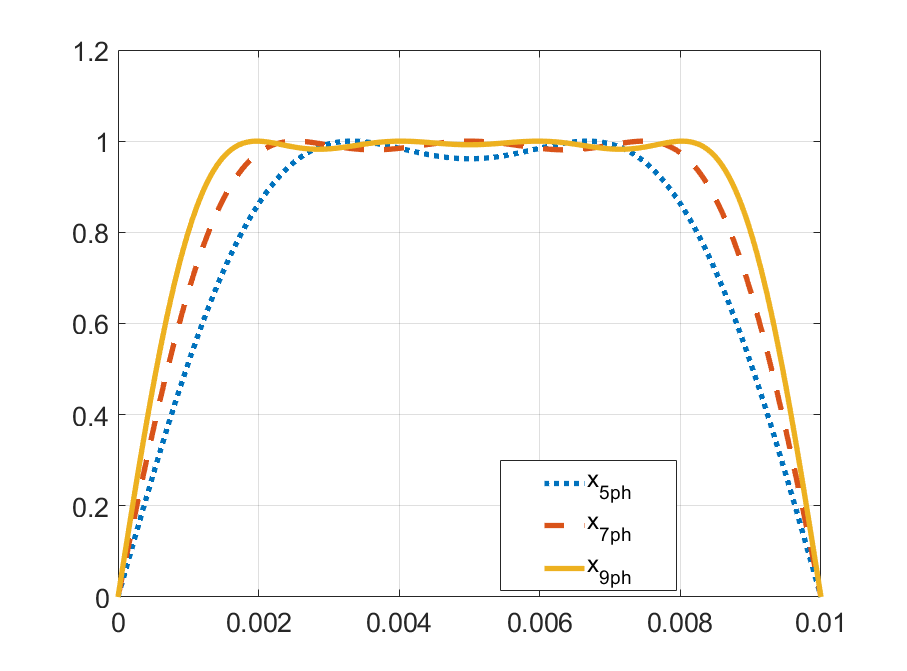
\includegraphics[width=6cm]{Figures/optimized_flux_waveform_5_7_9ph}
\caption{Figure example}
\label{fig:optimal-ratio-harmonics}
\end{figure}


\subsection{Traditional three-phase converters}

Conventional three-phase converters, correlation to SVPWM and 

\subsection{Three-phase four-leg converters}

Text text text. Text text text. Text text text. Text text text. Text
text text. Text text text. Text text text. Text text text. Text text
text. Text text text. Text text text. Text text text. Text text text.
Text text text. Text text text. Text text text. Text text text. Text
text text. Text text text. Text text text. Text text text.

\subsection{Multilevel converters}

Text text text. Text text text. Text text text. Text text text. Text
text text. Text text text. Text text text. Text text text. Text text
text. Text text text. Text text text. Text text text. Text text text.
Text text text. Text text text. Text text text. Text text text. Text
text text. Text text text. Text text text. Text text text.

\subsection{Multiphase converters}

Text text text. Text text text. Text text text. Text text text. Text
text text. Text text text. Text text text. Text text text. Text text
text. Text text text. Text text text. Text text text. Text text text.
Text text text. Text text text. Text text text. Text text text. Text
text text. Text text text. Text text text. Text text text.

\section{Experimental results}

Some experimental results.
\begin{figure}[!ht]
\begin{tabular}{>{\centering}p{4.2cm}>{\centering}p{4.2cm}}
\textcolor{red}{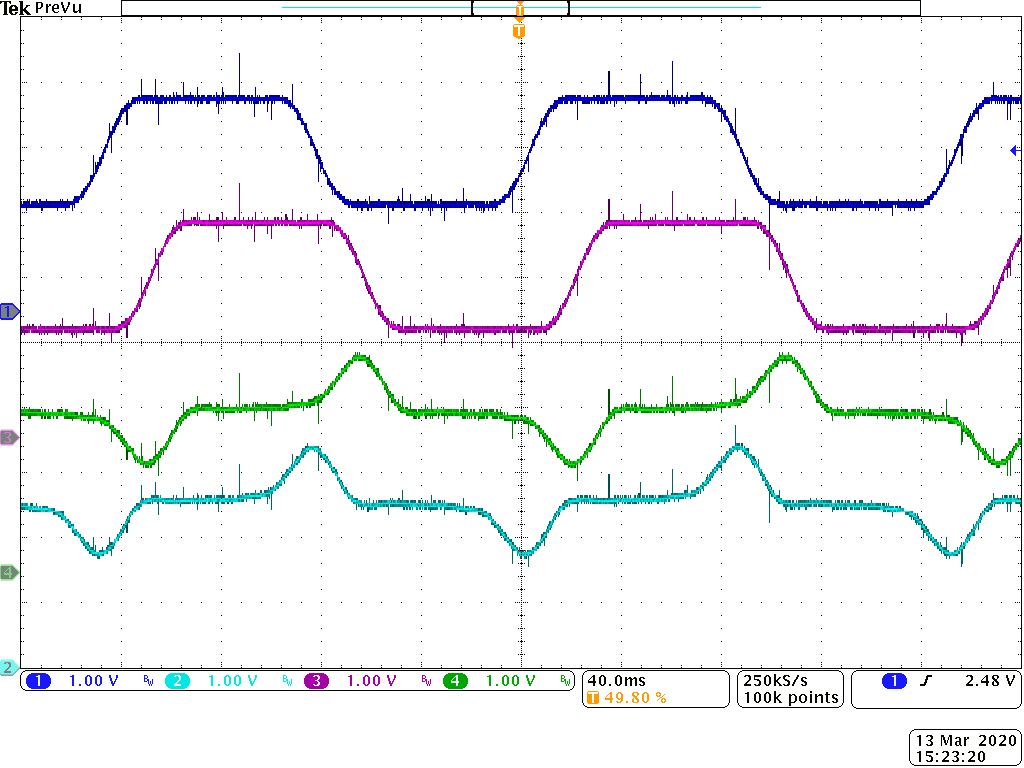
\includegraphics[width=0.48\columnwidth]{Figures/tek00002}} & \textcolor{red}{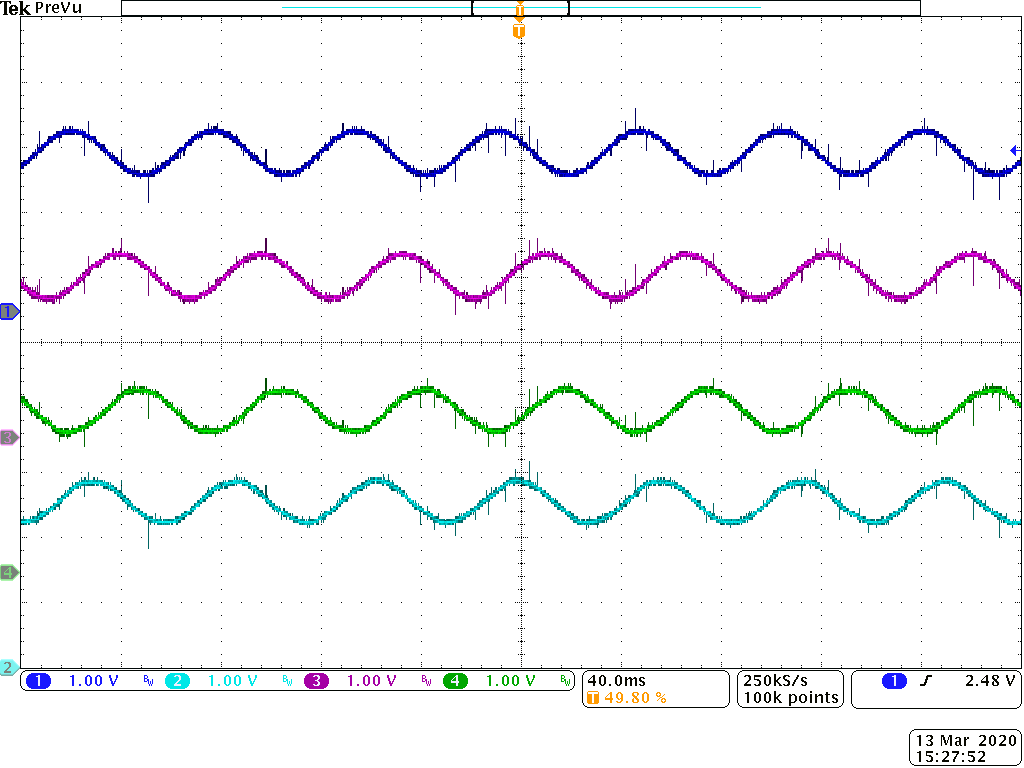
\includegraphics[width=0.48\columnwidth]{Figures/tek00002x}}\tabularnewline
 & \tabularnewline
{\footnotesize{}(a) Fundamental with 3\textsuperscript{rd} , 5\textsuperscript{th}
, and 7\textsuperscript{th} harmonic component.} & {\footnotesize{}(b) 3\textsuperscript{rd}harmonic component only.}\tabularnewline
\end{tabular}
\caption{Example of experimental results}
\label{fig:exp-results-1}
\end{figure}

\section{Conclusion}

Conclusion Text text text. Text text text. Text text text. Text text
text. Text text text. Text text text. Text text text. Text text text.
Text text text. Text text text..






\appendix


\section*{???}

Consider the interval
$$
 U_1 := \{u\mid -1\le u\le 1\}.
$$
Writing $u=u^+-u^-$ as the difference of its positive $u^+\ge 0$ and negative part $u^-\ge 0$, the previous set is connected with 
$$
 U_2 := \{(u^+,u^-)\mid -1\le u^+-u^-\le 1, u^+,u^-\ge 0\}.
$$
We depict $U_2$ in Figure \ref{fig:u2}.

\begin{figure}
 \centering
 
\begin{tikzpicture}
  \begin{axis}[ymin=-0.5,ymax=3,xmin=-0.5,xmax=3,minor tick num=1,axis lines = middle,xlabel=$x$,ylabel=$y$]
   \addplot [color=white,fill=blue,fill opacity=0.05] coordinates {(3,3) (2,3) (0,1) (0,0) (1,0) (3,2)};
   \addplot [thick,color=black] coordinates {(2,3) (0,1) (0,0) (1,0) (3,2)};
   \filldraw (axis cs: 0, 0) circle [radius=6];
   \filldraw (axis cs: 0, 1) circle [radius=6];
   \filldraw (axis cs: 1, 0) circle [radius=6];
  \end{axis}
 \end{tikzpicture}
 \caption{???}
 \label{fig:u2}
\end{figure}

While $U_1$ has two extremal points, $U_2$ has three extremal points. Even though these sets describe the same feasible set for optimization.

\section*{Acknowledgment}



\bibliographystyle{Bibliography/IEEEtranTIE}
\bibliography{Bibliography/ref}
%\bibliography{Bibliography/IEEEabrv,Bibliography/BIB_xx-TIE-xxxx}\ %IEEEabrv instead of IEEEfull

	
	
%\vspace{-1cm}
\begin{IEEEbiography}[{
\includegraphics[width=1in,height=1.25in,clip,keepaspectratio]{Figures/photo-men.eps}}]
{First A. Author1} and the other authors may include biographies at the end of regular papers. The first paragraph may contain a place and/or date of birth (list place, then date). Next, the author's educational background is listed. The degrees should be listed with type of degree in what field, which institution, city, state or country, and year degree was earned. The author's major field of study should be lower-cased.

The second paragraph uses the pronoun of the person (he or she) and not the author's last name. It lists military and work experience, including summer and fellowship jobs. Job titles are capitalized. The current job must have a location; previous positions may be listed without one. Information concerning previous publications may be included.

The third paragraph begins with the author's title and last name (e.g., Dr. Smith, Prof. Jones, Mr. Kajor, Ms. Hunter). List any memberships in professional societies other than the IEEE. Finally, list any awards and work for IEEE committees and publications. If a photograph is provided, the biography will be indented around it. The photograph is placed at the top left of the biography. Personal hobbies will be deleted from the biography.
\end{IEEEbiography}



\end{document}
